\documentclass[twoside]{book}

% Packages required by doxygen
\usepackage{fixltx2e}
\usepackage{calc}
\usepackage{doxygen}
\usepackage[export]{adjustbox} % also loads graphicx
\usepackage{graphicx}
\usepackage[utf8]{inputenc}
\usepackage{makeidx}
\usepackage{multicol}
\usepackage{multirow}
\PassOptionsToPackage{warn}{textcomp}
\usepackage{textcomp}
\usepackage[nointegrals]{wasysym}
\usepackage[table]{xcolor}

% Font selection
\usepackage[T1]{fontenc}
\usepackage[scaled=.90]{helvet}
\usepackage{courier}
\usepackage{amssymb}
\usepackage{sectsty}
\renewcommand{\familydefault}{\sfdefault}
\allsectionsfont{%
  \fontseries{bc}\selectfont%
  \color{darkgray}%
}
\renewcommand{\DoxyLabelFont}{%
  \fontseries{bc}\selectfont%
  \color{darkgray}%
}
\newcommand{\+}{\discretionary{\mbox{\scriptsize$\hookleftarrow$}}{}{}}

% Page & text layout
\usepackage{geometry}
\geometry{%
  a4paper,%
  top=2.5cm,%
  bottom=2.5cm,%
  left=2.5cm,%
  right=2.5cm%
}
\tolerance=750
\hfuzz=15pt
\hbadness=750
\setlength{\emergencystretch}{15pt}
\setlength{\parindent}{0cm}
\setlength{\parskip}{3ex plus 2ex minus 2ex}
\makeatletter
\renewcommand{\paragraph}{%
  \@startsection{paragraph}{4}{0ex}{-1.0ex}{1.0ex}{%
    \normalfont\normalsize\bfseries\SS@parafont%
  }%
}
\renewcommand{\subparagraph}{%
  \@startsection{subparagraph}{5}{0ex}{-1.0ex}{1.0ex}{%
    \normalfont\normalsize\bfseries\SS@subparafont%
  }%
}
\makeatother

% Headers & footers
\usepackage{fancyhdr}
\pagestyle{fancyplain}
\fancyhead[LE]{\fancyplain{}{\bfseries\thepage}}
\fancyhead[CE]{\fancyplain{}{}}
\fancyhead[RE]{\fancyplain{}{\bfseries\leftmark}}
\fancyhead[LO]{\fancyplain{}{\bfseries\rightmark}}
\fancyhead[CO]{\fancyplain{}{}}
\fancyhead[RO]{\fancyplain{}{\bfseries\thepage}}
\fancyfoot[LE]{\fancyplain{}{}}
\fancyfoot[CE]{\fancyplain{}{}}
\fancyfoot[RE]{\fancyplain{}{\bfseries\scriptsize Generated by Doxygen }}
\fancyfoot[LO]{\fancyplain{}{\bfseries\scriptsize Generated by Doxygen }}
\fancyfoot[CO]{\fancyplain{}{}}
\fancyfoot[RO]{\fancyplain{}{}}
\renewcommand{\footrulewidth}{0.4pt}
\renewcommand{\chaptermark}[1]{%
  \markboth{#1}{}%
}
\renewcommand{\sectionmark}[1]{%
  \markright{\thesection\ #1}%
}

% Indices & bibliography
\usepackage{natbib}
\usepackage[titles]{tocloft}
\setcounter{tocdepth}{3}
\setcounter{secnumdepth}{5}
\makeindex

% Hyperlinks (required, but should be loaded last)
\usepackage{ifpdf}
\ifpdf
  \usepackage[pdftex,pagebackref=true]{hyperref}
\else
  \usepackage[ps2pdf,pagebackref=true]{hyperref}
\fi
\hypersetup{%
  colorlinks=true,%
  linkcolor=blue,%
  citecolor=blue,%
  unicode%
}

% Custom commands
\newcommand{\clearemptydoublepage}{%
  \newpage{\pagestyle{empty}\cleardoublepage}%
}

\usepackage{caption}
\captionsetup{labelsep=space,justification=centering,font={bf},singlelinecheck=off,skip=4pt,position=top}

%===== C O N T E N T S =====

\begin{document}

% Titlepage & ToC
\hypersetup{pageanchor=false,
             bookmarksnumbered=true,
             pdfencoding=unicode
            }
\pagenumbering{alph}
\begin{titlepage}
\vspace*{7cm}
\begin{center}%
{\Large C\+PP }\\
\vspace*{1cm}
{\large Generated by Doxygen 1.8.13}\\
\end{center}
\end{titlepage}
\clearemptydoublepage
\pagenumbering{roman}
\tableofcontents
\clearemptydoublepage
\pagenumbering{arabic}
\hypersetup{pageanchor=true}

%--- Begin generated contents ---
\chapter{Class Index}
\section{Class List}
Here are the classes, structs, unions and interfaces with brief descriptions\+:\begin{DoxyCompactList}
\item\contentsline{section}{\hyperlink{classresultat}{resultat} \\*... blabla blabla }{\pageref{classresultat}}{}
\item\contentsline{section}{\hyperlink{classtexte}{texte} }{\pageref{classtexte}}{}
\end{DoxyCompactList}

\chapter{File Index}
\section{File List}
Here is a list of all documented files with brief descriptions\+:\begin{DoxyCompactList}
\item\contentsline{section}{/root/cpp/src/{\bfseries lib.\+h} }{\pageref{lib_8h}}{}
\item\contentsline{section}{/root/cpp/src/\hyperlink{mult_8h}{mult.\+h} \\*Description }{\pageref{mult_8h}}{}
\item\contentsline{section}{/root/cpp/src/{\bfseries text.\+h} }{\pageref{text_8h}}{}
\end{DoxyCompactList}

\chapter{Class Documentation}
\hypertarget{classresultat}{}\section{resultat Class Reference}
\label{classresultat}\index{resultat@{resultat}}


... blabla blabla  




{\ttfamily \#include $<$mult.\+h$>$}

\subsection*{Public Member Functions}
\begin{DoxyCompactItemize}
\item 
\mbox{\Hypertarget{classresultat_ac3f4984d7c159106135e1af82c9e4556}\label{classresultat_ac3f4984d7c159106135e1af82c9e4556}} 
int {\bfseries multiplication} (int num1, int num2)
\item 
int \hyperlink{classresultat_ac3f4984d7c159106135e1af82c9e4556}{multiplication} (int num1, int num2)
\item 
int \hyperlink{classresultat_a390b2d3477982b10e1b36fc52ba102ea}{addition} (int num3, int num4)
\item 
int \hyperlink{classresultat_ab1dfe27df49fb99860cc7cbf03ad19d9}{division} (int num5, int num6)
\end{DoxyCompactItemize}


\subsection{Detailed Description}
... blabla blabla 

\subsection{Member Function Documentation}
\mbox{\Hypertarget{classresultat_a390b2d3477982b10e1b36fc52ba102ea}\label{classresultat_a390b2d3477982b10e1b36fc52ba102ea}} 
\index{resultat@{resultat}!addition@{addition}}
\index{addition@{addition}!resultat@{resultat}}
\subsubsection{\texorpdfstring{addition()}{addition()}}
{\footnotesize\ttfamily int resultat\+::addition (\begin{DoxyParamCaption}\item[{int}]{num3,  }\item[{int}]{num4 }\end{DoxyParamCaption})}

brief... 
\begin{DoxyParams}{Parameters}
{\em addition} & description... \\
\hline
\end{DoxyParams}
\mbox{\Hypertarget{classresultat_ab1dfe27df49fb99860cc7cbf03ad19d9}\label{classresultat_ab1dfe27df49fb99860cc7cbf03ad19d9}} 
\index{resultat@{resultat}!division@{division}}
\index{division@{division}!resultat@{resultat}}
\subsubsection{\texorpdfstring{division()}{division()}}
{\footnotesize\ttfamily int resultat\+::division (\begin{DoxyParamCaption}\item[{int}]{num5,  }\item[{int}]{num6 }\end{DoxyParamCaption})}

brief... 
\begin{DoxyParams}{Parameters}
{\em division} & description... \\
\hline
\end{DoxyParams}
\mbox{\Hypertarget{classresultat_ac3f4984d7c159106135e1af82c9e4556}\label{classresultat_ac3f4984d7c159106135e1af82c9e4556}} 
\index{resultat@{resultat}!multiplication@{multiplication}}
\index{multiplication@{multiplication}!resultat@{resultat}}
\subsubsection{\texorpdfstring{multiplication()}{multiplication()}}
{\footnotesize\ttfamily int resultat\+::multiplication (\begin{DoxyParamCaption}\item[{int}]{num1,  }\item[{int}]{num2 }\end{DoxyParamCaption})}

brief... 
\begin{DoxyParams}{Parameters}
{\em multiplication} & description... \\
\hline
\end{DoxyParams}


The documentation for this class was generated from the following files\+:\begin{DoxyCompactItemize}
\item 
/root/cpp/src/lib.\+h\item 
/root/cpp/src/\hyperlink{mult_8h}{mult.\+h}\item 
/root/cpp/src/lib.\+cpp\item 
/root/cpp/src/mult.\+cpp\end{DoxyCompactItemize}

\hypertarget{classtexte}{}\section{texte Class Reference}
\label{classtexte}\index{texte@{texte}}
\subsection*{Public Member Functions}
\begin{DoxyCompactItemize}
\item 
\mbox{\Hypertarget{classtexte_acdc1e996628c96dc4d2b0ad7e4ce802f}\label{classtexte_acdc1e996628c96dc4d2b0ad7e4ce802f}} 
void {\bfseries hello} ()
\item 
\mbox{\Hypertarget{classtexte_a637e30a95893ab0246b1bd0faff35b86}\label{classtexte_a637e30a95893ab0246b1bd0faff35b86}} 
void {\bfseries bonjour} ()
\item 
\mbox{\Hypertarget{classtexte_afa0e63c849bab06ba927e447cb4dada3}\label{classtexte_afa0e63c849bab06ba927e447cb4dada3}} 
void {\bfseries cava} ()
\end{DoxyCompactItemize}


The documentation for this class was generated from the following files\+:\begin{DoxyCompactItemize}
\item 
/root/cpp/src/text.\+h\item 
/root/cpp/src/text.\+cpp\end{DoxyCompactItemize}

\chapter{File Documentation}
\hypertarget{mult_8h}{}\section{/root/cpp/src/mult.h File Reference}
\label{mult_8h}\index{/root/cpp/src/mult.\+h@{/root/cpp/src/mult.\+h}}


description  


{\ttfamily \#include $<$iostream$>$}\newline
Include dependency graph for mult.\+h\+:\nopagebreak
\begin{figure}[H]
\begin{center}
\leavevmode
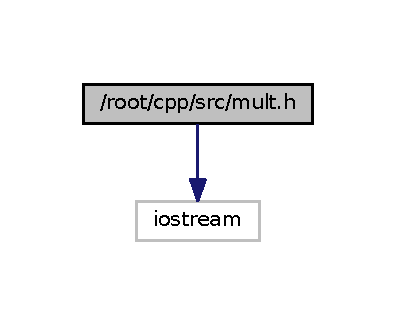
\includegraphics[width=190pt]{mult_8h__incl}
\end{center}
\end{figure}
\subsection*{Classes}
\begin{DoxyCompactItemize}
\item 
class \hyperlink{classresultat}{resultat}
\begin{DoxyCompactList}\small\item\em ... blabla blabla \end{DoxyCompactList}\end{DoxyCompactItemize}


\subsection{Detailed Description}
description 

\begin{DoxyAuthor}{Author}
prenom version 
\end{DoxyAuthor}

%--- End generated contents ---

% Index
\backmatter
\newpage
\phantomsection
\clearemptydoublepage
\addcontentsline{toc}{chapter}{Index}
\printindex

\end{document}
